\documentclass[aspectratio=169,11pt]{beamer}

% Moderne Pakete
\usepackage[ngerman]{babel}
\usepackage[utf8]{inputenc}
\usepackage[T1]{fontenc}
\usepackage{lmodern}
\usepackage{siunitx}
\usepackage{mhchem}
\usepackage{tabularray}
\usepackage[backend=biber,style=numeric,sorting=none]{biblatex}
\addbibresource{../bib/references.bib}\usepackage{graphicx}
\usepackage{tikz}
\usepackage{pgfplots}
\pgfplotsset{compat=1.18}
\usepackage{hyperref}
\usepackage{colortbl}
\usepackage{booktabs}
\usepackage{amsmath,amssymb}
\usepackage{ragged2e}

% THGA Farben gemäß Corporate Design
\definecolor{thgablue}{RGB}{0,60,124}       % Hauptfarbe Blau
\definecolor{thgared}{RGB}{227,0,15}        % Hauptfarbe Rot
\definecolor{thgagreen}{RGB}{105,192,172}   % Hauptfarbe Grün
\definecolor{thgadarkgreen}{RGB}{31,102,85}   	% Dunkelgrün
\definecolor{thgalightgreen}{RGB}{163,217,204}   % Hellgrün
\definecolor{thgadarkblue}{RGB}{0,37,76}    % Dunkelblau
\definecolor{thgalightblue}{RGB}{204,229,255} % Hellblau
\definecolor{thgadarkred}{RGB}{153,0,10}  % Dunkelrot
\definecolor{thgalightred}{RGB}{229,207,208}  % Hellrot
\definecolor{thgadarkgray}{RGB}{51,52,53} % Dunkelgrau
\definecolor{thgagray}{RGB}{102,103,104}    % Grau
\definecolor{thgalightgray}{RGB}{225,226,227} % Hellgrau
\definecolor{thgadarkyellow}{RGB}{179,146,18} % Dunkelgelb
\definecolor{thgalightyellow}{RGB}{252,231,148} % Hellgelb

% Beamer Theme - minimalistisch
\usetheme{default}
\usecolortheme{default}

% Entferne alle Schatten und 3D-Effekte
\setbeamertemplate{blocks}[default]
\setbeamertemplate{items}[square]
\setbeamertemplate{sections/subsections in toc}[square]
\setbeamertemplate{title page}[default]
\setbeamertemplate{frametitle}[default]

% Farben anpassen - flaches Design
\setbeamercolor{structure}{fg=thgablue}
\setbeamercolor{frametitle}{bg=thgablue,fg=white}
\setbeamercolor{title}{fg=thgablue}
\setbeamercolor{title in head/foot}{fg=thgagray}
\setbeamercolor{subtitle}{fg=thgagray}
\setbeamercolor{author}{fg=thgagreen}
\setbeamercolor{author in head/foot}{fg=thgagray}
\setbeamercolor{institute}{fg=thgalightgreen}
\setbeamercolor{date}{fg=thgalightgreen}
\setbeamercolor{date in head/foot}{fg=thgagray}
\setbeamercolor{section in toc}{fg=thgablue}
\setbeamercolor{subsection in toc}{fg=thgagray}
\setbeamercolor{itemize item}{fg=thgablue}
\setbeamercolor{itemize subitem}{fg=thgagreen}
\setbeamercolor{enumerate item}{fg=thgablue}
\setbeamercolor{subitem}{fg=thgagreen}
\setbeamercolor{block title}{bg=thgablue,fg=white}
\setbeamercolor{block body}{bg=thgalightgray,fg=black}
\setbeamercolor{block title alerted}{bg=thgared,fg=white}
\setbeamercolor{block body alerted}{bg=thgalightred,fg=black}
\setbeamercolor{block title example}{bg=thgagreen,fg=white}
\setbeamercolor{block body example}{bg=thgalightblue,fg=black}

% Schriftarten
\setbeamerfont{title}{size=\LARGE,series=\bfseries}
\setbeamerfont{subtitle}{size=\large}
\setbeamerfont{frametitle}{size=\Large,series=\bfseries}
\setbeamerfont{framesubtitle}{size=\normalsize}
\setbeamerfont{author}{size=\normalsize}
\setbeamerfont{institute}{size=\small}
\setbeamerfont{date}{size=\small}

% Navigation ausblenden
\setbeamertemplate{navigation symbols}{}

% Fußzeile
\setbeamertemplate{footline}{
    \hbox{%
    \hspace*{0.25cm}
    \begin{beamercolorbox}[wd=.2\paperwidth,ht=2.5ex,dp=1ex,left]{author in head/foot}%
        \usebeamerfont{author in head/foot}\hspace*{2ex}\insertshortdate
    \end{beamercolorbox}%
    \begin{beamercolorbox}[wd=.50\paperwidth,ht=2.5ex,dp=1ex,center]{title in head/foot}%
        \usebeamerfont{title in head/foot}\insertshorttitle
    \end{beamercolorbox}%
    \begin{beamercolorbox}[wd=.26\paperwidth,ht=2.5ex,dp=1ex,right]{date in head/foot}%
        \usebeamerfont{date in head/foot}
        \insertframenumber{} / \inserttotalframenumber\hspace*{2ex}
    \end{beamercolorbox}}%
}

% Titelseite
\setbeamertemplate{title page}{
    \vbox{}
    \vfill
    \begin{columns}[b]
        \begin{column}{0.35\textwidth}
            \hspace*{-1cm}\vspace*{-1cm}
\includegraphics[width=6cm]{../img/Logo_cmyk_4c_300DPI_crop} 
        \end{column}
        \begin{column}{0.6\textwidth}
            \raggedright
            %\hspace{}
            \begin{beamercolorbox}[sep=8pt,left]{title}
                \usebeamerfont{title}\inserttitle\par%
            \end{beamercolorbox}%
            \vskip-0.25em%
            \begin{beamercolorbox}[sep=8pt,left]{subtitle}
                \usebeamerfont{subtitle}\insertsubtitle\par%
            \end{beamercolorbox}%
            \vskip2em%
            \begin{beamercolorbox}[sep=8pt,left]{author}
                \usebeamerfont{author}\insertauthor
            \end{beamercolorbox}
            \vskip-1em%
            \begin{beamercolorbox}[sep=8pt,left]{institute}
                \usebeamerfont{institute}\insertinstitute
            \end{beamercolorbox}
            \vskip-1em%
            \begin{beamercolorbox}[sep=8pt,left]{date}
                \usebeamerfont{date}\insertdate
            \end{beamercolorbox}
        \end{column}
    \end{columns}
    \vfill
}

% Folienrahmen
\setbeamertemplate{frametitle}{
  \nointerlineskip
  \begin{beamercolorbox}[wd=\paperwidth,ht=1.2cm,dp=0.3cm]{frametitle}
    \begin{minipage}[c][1.5cm][c]{0.8\paperwidth}
      \vspace*{-0.55cm}
      \hspace*{0.5cm}%
      \usebeamerfont{frametitle}\insertframetitle\par
      \hspace*{0.5cm}%
      \usebeamerfont{framesubtitle}%
      \usebeamercolor[fg]{framesubtitle}%
      \insertframesubtitle\hspace*{-1pt}\null
    \end{minipage}%
    \begin{minipage}[c][1.5cm][c]{0.2\paperwidth}
      \raggedleft
      \raisebox{0.65cm}{%
        
\includegraphics[height=1.2cm]{../img/Logo_cmyk_negativ}%
      }\hspace*{1cm}
    \end{minipage}
  \end{beamercolorbox}
}

% Texteinzug definieren
\setbeamersize{text margin left=0.5cm, text margin right=1cm}


% Umgebung für Definitionen
\newenvironment{flatbox}[2][thgablue]{%
    \begin{tikzpicture}
    \node[
        draw=#1,
        fill=#1!10,
        line width=2pt,
        rounded corners=2pt,
        inner xsep=10pt,
        inner ysep=10pt,
        text width=\textwidth - 20pt,
        minimum width=\textwidth - 4pt,
        anchor=north west
    ] (box) \bgroup
    \begin{minipage}{\textwidth}
    \justifying
    \textcolor{#1}{\textbf{#2}}\\[0.5em]
}{%
    \end{minipage}
    \egroup;
    \end{tikzpicture}
}

% Befehle für farbige Hervorhebungen
\newcommand{\thgablue}[1]{\textcolor{thgablue}{#1}}
\newcommand{\thgared}[1]{\textcolor{thgared}{#1}}
\newcommand{\thgagreen}[1]{\textcolor{thgagreen}{#1}}
\newcommand{\thgadarkblue}[1]{\textcolor{thgadarkblue}{#1}}
\newcommand{\thgadarkred}[1]{\textcolor{thgadarkred}{#1}}
\newcommand{\thgadarkgreen}[1]{\textcolor{thgadarkgreen}{#1}}
\newcommand{\thgadarkgray}[1]{\textcolor{thgadarkgray}{#1}}
\newcommand{\thgadarkyellow}[1]{\textcolor{thgadarkyellow}{#1}}

% Informationen zum Vortrag
\title{Lehre als Dialog mit dem Code}
\subtitle{Jupyter Notebooks im Ingenieurstudium}
\author{Prof. Dr.-Ing. Robin Wegge}
\institute{Technische Hochschule Georg Agricola}
\date{Best Practice Lehre 2025}

\begin{document}
%%%%%%%%%%%%%%%%%%%%%%I N H A L T%%%%%%%%%%%%%%%%%%%%%%%%%
% Titelfolie
\begin{frame}[plain]
    \maketitle
\end{frame}

\begin{frame}{Agenda}
\tableofcontents
\end{frame}


% Eingangsthese
\begin{frame}{Kompetenzverschiebung in der Ingenieurausbildung}
\framesubtitle{Warum klassische Lehransätze nicht mehr ausreichen \cite{siemens2013}}
\section{Kompetenzverschiebung in der Ingenieurausbildung}
    \begin{center}
        \begin{tikzpicture}
            \node[
                draw=thgadarkblue,
                fill=thgalightblue,
                line width=3pt,
                rounded corners=5pt,
                inner sep=10pt,
                text width=0.9\textwidth,
                align=center
            ] {
                \Large\textbf{\thgadarkblue{
                \begin{tabular}{@{}c@{}}
                Studierende rechnen mit vereinfachten\\[0.2em]
                Modellen und idealen Randbedingungen. \\[0.6em]
                Die Berufspraxis erfordert den Umgang\\[0.2em]
                mit komplexen digitalen Systemen.
                \end{tabular}
                }}
            };
        \end{tikzpicture}
    \end{center}
\end{frame}

% Problemstellung
\begin{frame}{Typische Aufgabenstellung}
    \framesubtitle{Dimensionierung eines Windparks}
    \textbf{Aufgabe:} Dimensionieren Sie einen Windpark für eine Fläche von \qty{1}{\kilo\meter\squared}
    \begin{columns}[T]
    \hspace*{-0.15cm}
        \begin{column}{0.45\textwidth}          
            \vspace{0.25em}
            \textbf{Gegebene Parameter}
            \begin{itemize}
                \item Anlagentyp: \qty{2}{\mega\watt} Nennleistung
                \item Rotordurchmesser: \qty{100}{\meter}
                \item Leistungsbeiwert: \qty{50}{\percent}
                \item Verfügbarkeit: \qty{95}{\percent}
                \item Windgeschwindigkeit: \qty{8}{\meter\per\second}
            \end{itemize}
            
            \vspace{0.25em}
            \textbf{Gegebene Gleichungen}
            \begin{align*}
            	P_{\text{WKA}} &= \frac{1}{2} \cdot \eta \cdot c_\text{p} \cdot \rho_\text{L} \cdot A_{\text{WKA}} \cdot v^3  \\
            	P_\text{ges} &= n \cdot P_\text{WKA}  \cdot \text{Verfügbarkeit}
            \end{align*}
        \end{column}
        
        \begin{column}{0.55\textwidth}
        \vspace*{0.75cm}
            \begin{tikzpicture}[scale=0.85]
            \tikzset{
                windrad/.pic={
                    \draw[blue, thick] (0,0) circle (0.3);
                    \foreach \angle in {90, 210, 330} {
                        \begin{scope}[rotate=\angle]
                            \draw[blue, thick, fill=blue!20]
                                (0,0) -- (0.05,0.15)
                                .. controls (0,0.3) .. (-0.05,0.15)
                                -- cycle;
                        \end{scope}
                    }
                }
            }
            
            \draw[help lines, step=1, gray!60] (0,0) grid (4,4);
            \draw[gray, dashed, thick] (0,0) rectangle (4,4);
            \node[anchor=north west] at (0,4.65) {\small $1\,\text{km}^2$};
            
            \foreach \x/\y in {1/1, 3/1, 1/3, 3/3} {
                \pic at (\x,\y) {windrad};
            }
            
            \draw[-] (3,1) -- (5,0.5)
                node[below right] {\small Windkraftanlage};
            
            \draw[<->] (1,-0.5) -- (3,-0.5)
                node[midway, below] {\small $5 \cdot d_\text{R}$};
            \draw[<->] (-0.5,1) -- (-0.5,3)
                node[midway,
                    rotate=90,
                    anchor=south,
                    xshift=-0.4cm,
                    xshift=0.45cm] 
                    {\small $5 \cdot d_\text{R}$};
            
            \begin{scope}[shift={(6,3)}]
                \draw[red, thick, fill=red!10]
                    (-0.15,-1) -- (-0.05,0) -- (0.05,0) -- (0.15,-1) -- cycle;
                
                \draw[red, thick] (0,0) circle (0.5);
                \foreach \angle in {90, 210, 330} {
                    \begin{scope}[rotate=\angle]
                        \draw[red, thick, fill=red!20]
                            (0,0) -- (0.07,0.25)
                            .. controls (0,0.5) .. (-0.07,0.25)
                            -- cycle;
                    \end{scope}
                }
                
                \draw[->] (0,0) -- (0.5,0)
                    node[midway, xshift=0.6cm] {\small $\frac{d_\text{R}}{2}$};
                
                \node[below] at (0.5,-1) {\small Rotorfläche $A_\text{WKA}$};
            \end{scope}
        \end{tikzpicture}
            
        \end{column}
    \end{columns}
\end{frame}

\begin{frame}{Die Realität}
	\framesubtitle{Komplexe Topografien und wechselnde Wetterverhältnisse}
  		Als Ingenieur*in planen Sie einen Windpark für eine Fläche von \qty{1}{\kilo\meter\squared} \\ [1em]
    \begin{columns}[T]
    	\begin{column}{0.66\textwidth}
    			\textbf{Topografie} \\
    			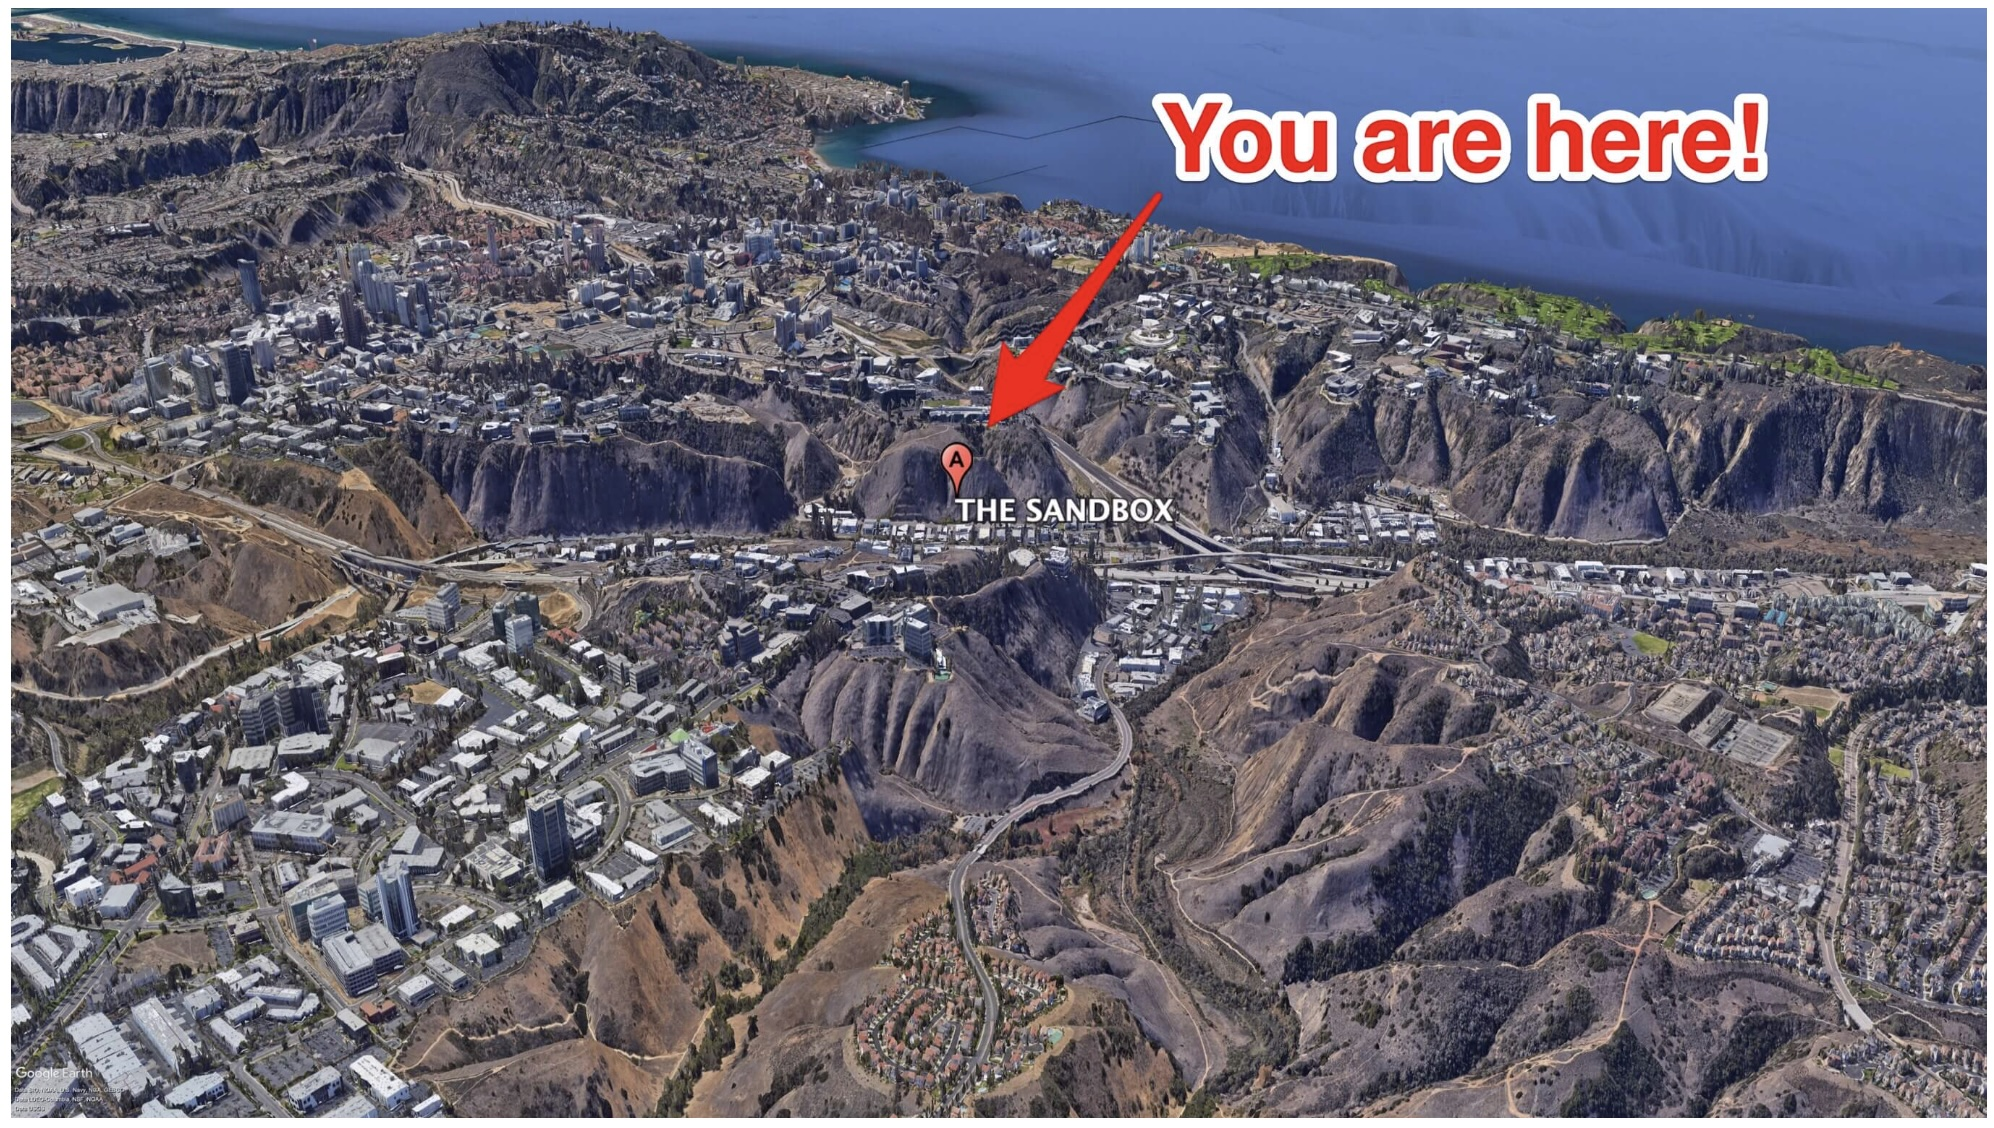
\includegraphics[width=1.\linewidth]{../img/you_are_here}
		\end{column}
    		
    	\begin{column}{0.33\textwidth}
    		\textbf{Windgeschwindigkeit} \\
    		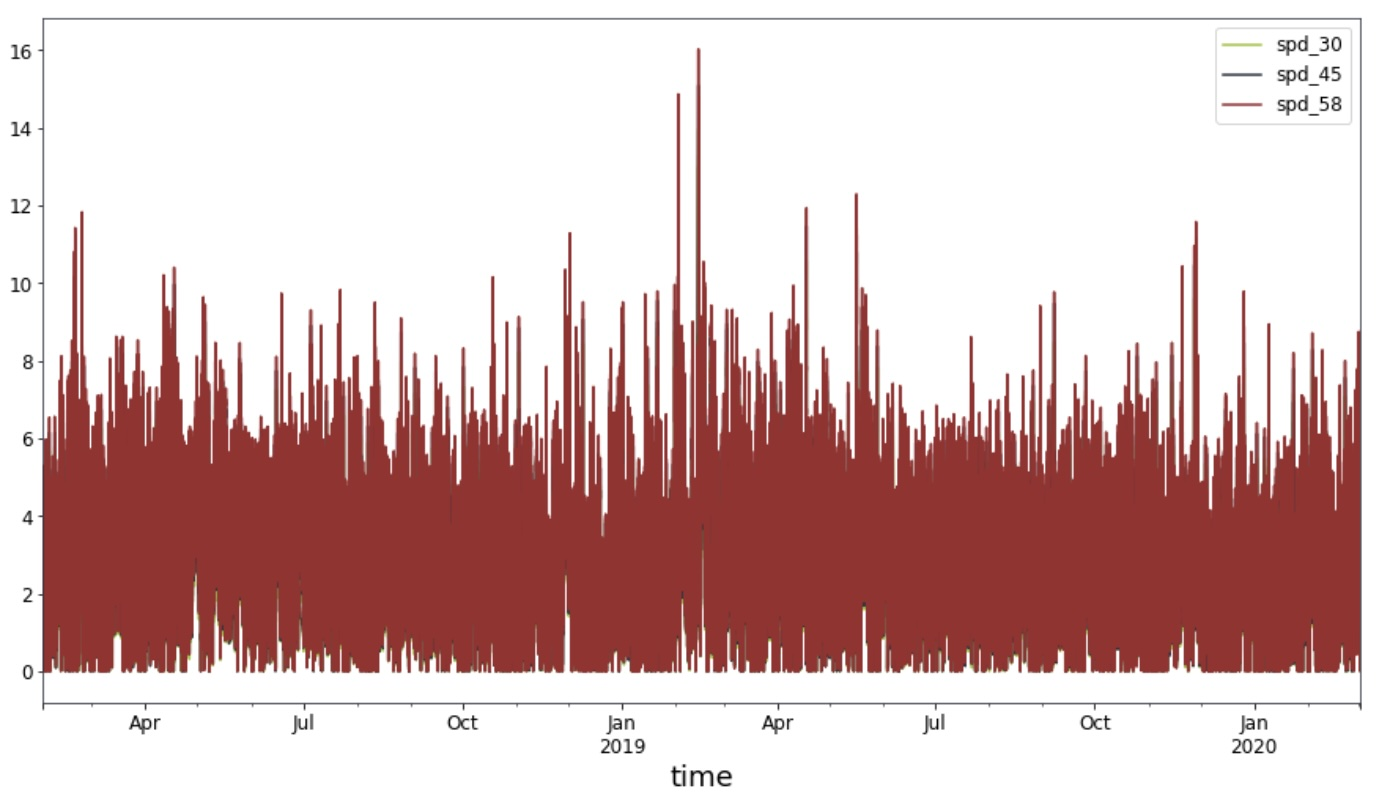
\includegraphics[width=0.75\linewidth]{../img/speed}
  			\textbf{Windrichtung} \\
    		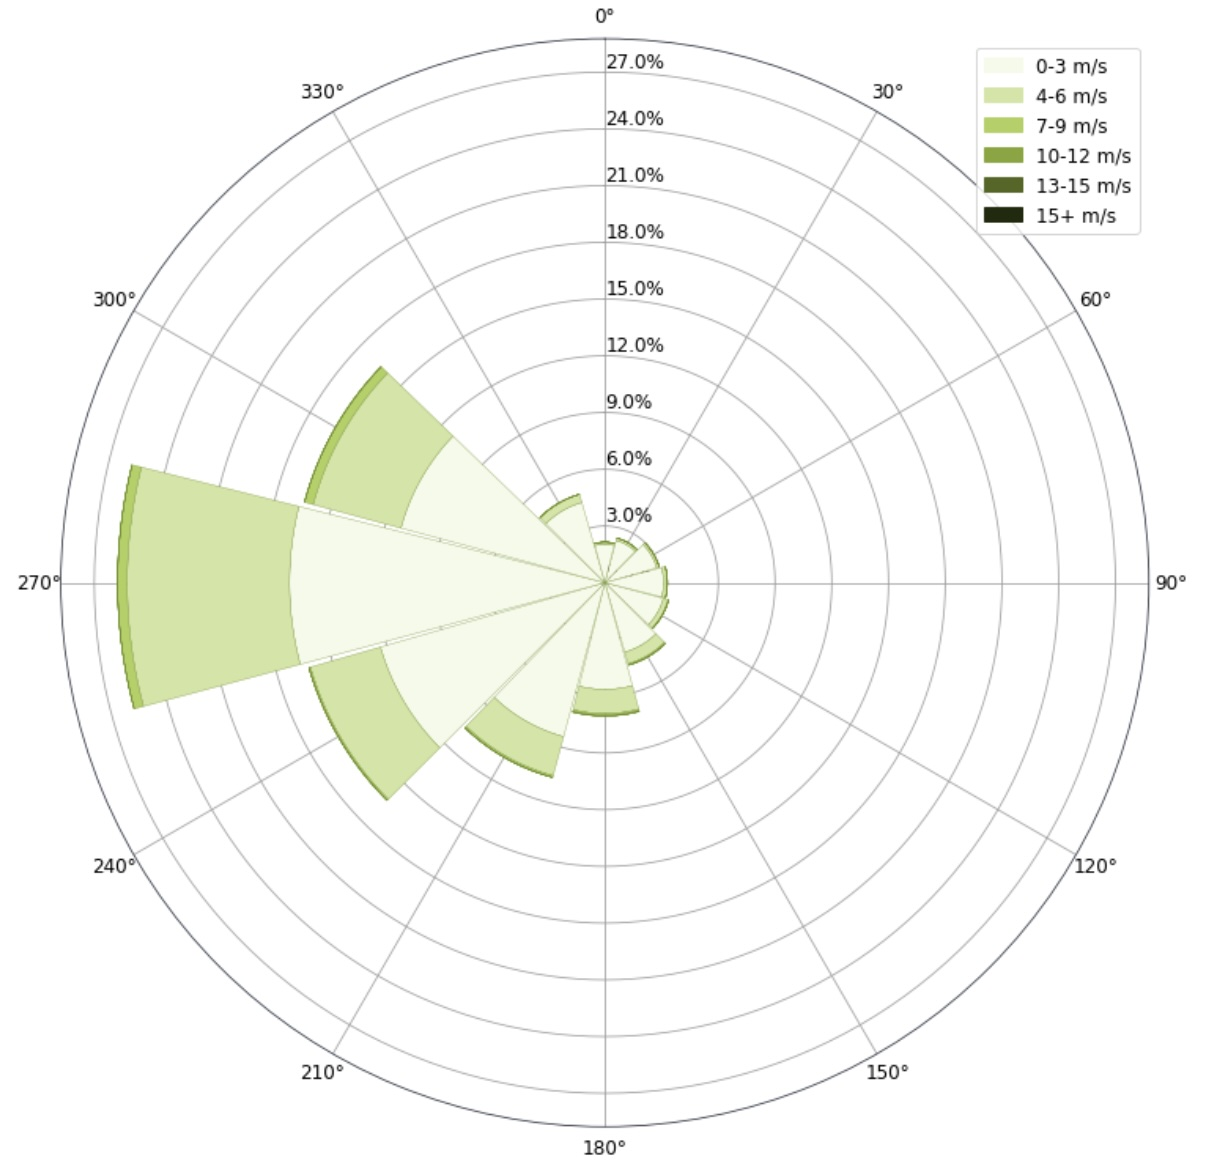
\includegraphics[height=0.3\textheight]{../img/direction}
		\end{column}
    \end{columns}
\end{frame}

\begin{frame}{Vom Plan zur Realität}
	\framesubtitle{Komplexe Projektierung erfordert interdisziplinäres Denken}
  		Als Ingenieur*in planen Sie einen Windpark für eine Fläche von \qty{1}{\kilo\meter\squared} \\ [1em]
    \begin{columns}[T]
    	\begin{column}<1->{0.66\textwidth}
   			\textbf{Basic Engineering} \\
   			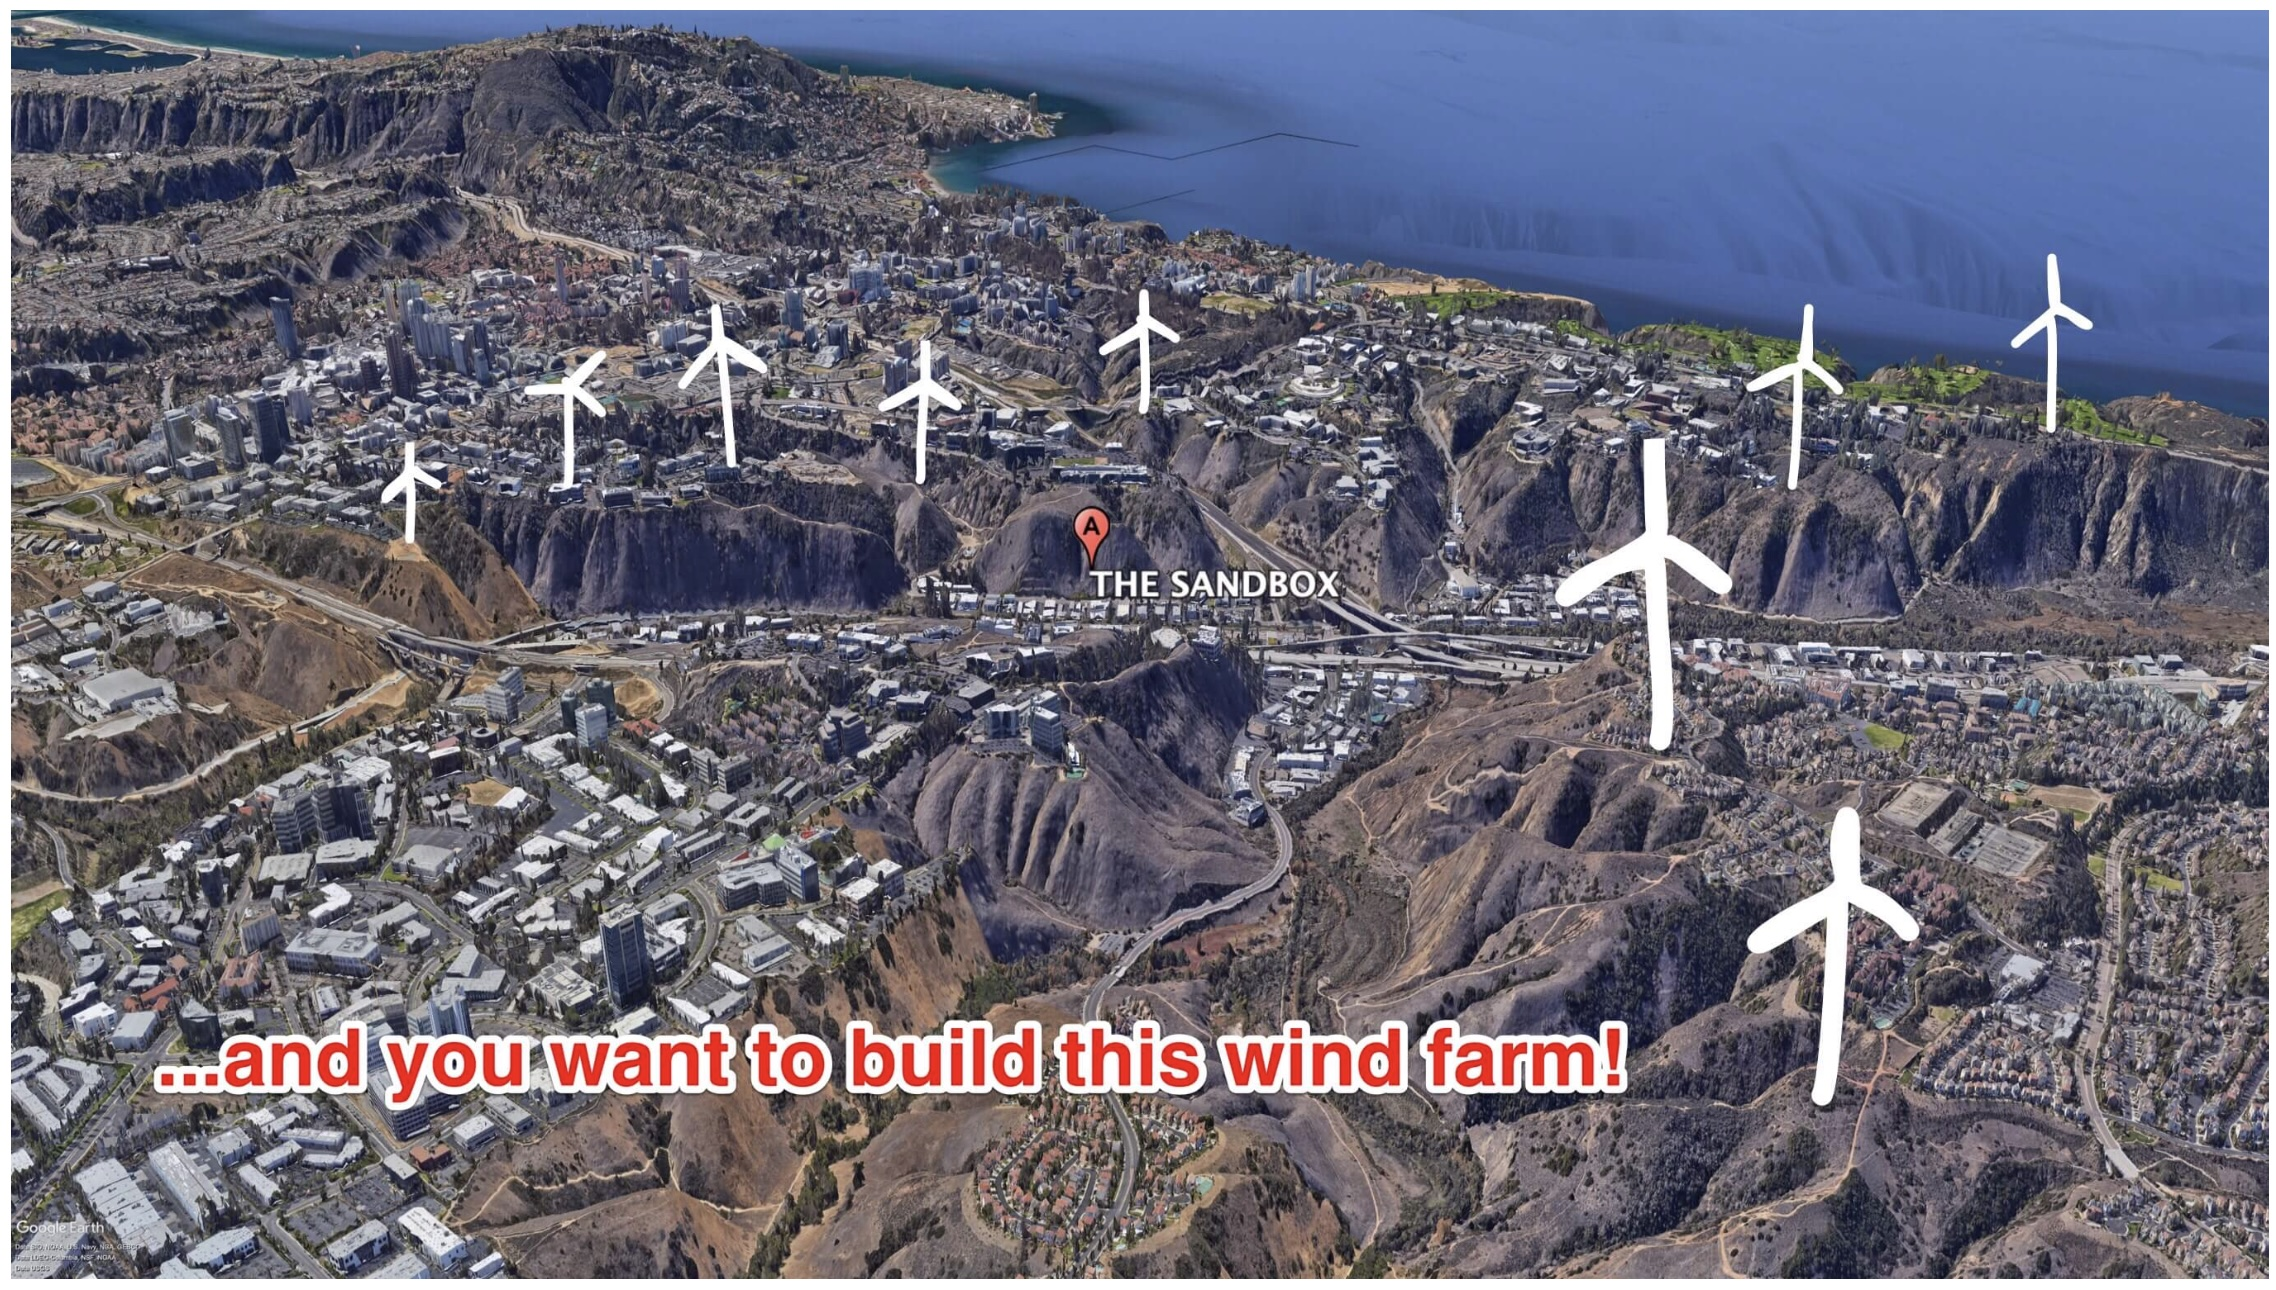
\includegraphics[width=1.\linewidth]{../img/planning_a_windfarm}
		\end{column}
    		
    	\begin{column}<2->{0.33\textwidth}
    		\textbf{Project Assessment} \\
    		
\includegraphics[width=1.\linewidth]{../img/meme}
		\end{column}
    \end{columns}
\end{frame}

\begin{frame}{Grenzen vereinfachter Modellierung}
	\framesubtitle{Daten bestimmen die Entscheidungsfindung}
    \begin{columns}[T]
    	\begin{column}{0.45\textwidth}
    	\vspace*{0.75cm}
   			\textbf{Reale Einflussfaktoren}
            \begin{itemize}
                \item Zeitlich variable Windverhältnisse
                \item Komplexe Strömungsmuster
                \item Nachlaufeffekte zwischen Anlagen
                \item Topografische Einflüsse
                \item Wartungsintervalle und Ausfälle
                \item Netzintegration und Regelstrategien
            \end{itemize}
		\end{column}
    		
    	\begin{column}{0.55\textwidth}
    		\begin{center}
        	\begin{tikzpicture}
            	\node[
                	draw=thgadarkgray,
           		    fill=thgalightgray,
           	     	line width=3pt,
        	        rounded corners=5pt,
            	    inner sep=10pt,
                	text width=0.9\textwidth,
	                align=center
    	        ] {
        	        \textbf{\thgadarkgray{
        	        \begin{tabular}{@{}c@{}}                
            	    Reale Aufgaben erfordern \\[0.2em]
            	    digitale Werkzeuge. \\[0.6em]
                	\emph{Ingenieurwissenschaftliches Arbeiten} \\[0.2em]
                	bedeutet heute: Analyse und\\[0.2em]
                	Visualisierung komplexer Datenmengen.
        	        \end{tabular}
        	        }}
            	};
	        \end{tikzpicture}
    	\end{center}
		\end{column}
    \end{columns}
    
    \begin{center}
    
    \begin{tikzpicture}
		\node[
			  draw=thgadarkyellow,
			  fill=thgalightyellow,
			  line width=3pt,
			  rounded corners=5pt,
			  inner sep=10pt,
			  text width=0.9\textwidth,
			  align=center
    	      ] {
    	      \textbf{\thgadarkyellow{
    	      $\Rightarrow$ Data Literacy ist Kernkompetenz moderner Ingenieure und Ingeneurinnen!
    	      }}
             };
	\end{tikzpicture}
	\end{center}
	
\end{frame}

\begin{frame}{Data Lit...?}
	\centering
	
\includegraphics[height=0.8\textheight]{../img/9yvfq8}
\end{frame}

\begin{frame}{Data LitERACY!}
\framesubtitle{Datenkompetenz als Schlüsselqualifikation}
\section{Integration von Data Literacy im Ingenieurstudium}    
    \begin{center}
    \begin{minipage}[c]{0.4\textwidth}
        \centering
        
\includegraphics[height=0.45\textheight]{../img/9yvfq8}
    \end{minipage}
    \hspace{1cm}
    \begin{minipage}[c]{0.5\textwidth}
    	\begin{flatbox}[thgablue]{Definition \cite{ridsdale2015}}
			Datenkompetenz bezeichnet die Fähigkeit, Daten zu lesen, zu verstehen, zu erstellen und zu kommunizieren. \\ Sie umfasst das kritische Denken im Umgang mit Daten sowie die Kompetenz, datengestützte Entscheidungen zu treffen.
		\end{flatbox}
    \end{minipage}
    \end{center}
\end{frame}





\begin{frame}{Integration in die Ingenieurausbildung}
    \framesubtitle{Anforderungen an moderne Lehr-Lern-Umgebungen}
    \vspace*{0.5em}
   	
	\begin{flatbox}[thgared]{Programmieren ist Mittel zum Zweck}
		Das Ziel ist der Aufbau einer Methodenkompetenz zur Analyse, Bewertung und Gestaltung komplexer technischer Systeme entwickeln. Nicht perfekte Programmierer*innen auszubilden.
	\end{flatbox}
    \vspace{-1.25em}
    
    \begin{columns}<2->[T]
        \begin{column}{0.48\textwidth}
            \textbf{\thgablue{Technische Anforderungen}}
            \begin{itemize}
                \item<2-> Zugriff auf reale Datensätze
                \item<2-> Professionelle Entwicklungsumgebung
                \item<2-> Leistungsfähige Visualisierung
                \item<2-> Wissenschaftliche Bibliotheken
                \item<2-> Reproduzierbare Workflows
            \end{itemize}
        \end{column}
        \begin{column}{0.48\textwidth}
            \textbf{\thgagreen{Didaktische Anforderungen}}
            \begin{itemize}
                \item<2-> Authentische Problemstellungen
                \item<2-> Exploratives Lernen fördern
                \item<2-> Direktes Feedback ermöglichen
                \item<2-> Schrittweise Komplexitätssteigerung
                \item<2-> Dokumentation des Lernprozesses
            \end{itemize}
        \end{column}
    \end{columns}
\end{frame}


\begin{frame}{Die Lösung: Jupyter Notebooks \cite{kluyver2016, barba2023}}
\framesubtitle{Integrierte Umgebung für Code, Dokumentation und Visualisierung}
\section{Jupyter Notebooks als Lehr-Lern-Umgebung} 
    \begin{columns}[T]
    \hspace*{-0.5cm}
        \begin{column}{0.55\textwidth}
            \textbf{Was sind Jupyter Notebooks?}
            \begin{itemize}
                \item Webbasierte Entwicklungsumgebung
                \item Integration von Code, Text und Grafiken
                \item Zellbasierte, interaktive Ausführung
                \item Sofortige Visualisierung der Ergebnisse
            \end{itemize}
            
            \vspace{0.5em}
            \textbf{Vorteile für die Lehre}
            \begin{itemize}
                \item Niedrigschwelliger Einstieg
                \item Narrative Strukturierung möglich
                \item Reproduzierbare Analysen
                \item Kollaboratives Arbeiten
            \end{itemize}
        \end{column}
        \begin{column}{0.4\textwidth}
            \begin{center}
                \includegraphics[width=\textwidth]{../img/jupyter_screenshot}
            \end{center}
        \end{column}
    \end{columns}
\end{frame}

\begin{frame}[plain]
    \begin{center}
    \vfill
    
    \href{http://localhost:8888/lab/tree/Users/robin/Nextcloud/90\%20Academia/10\%20Vortra\%CC\%88ge/2025-06-30\%20Best\%20Practice\%20Lehre/05\%20Demo}{%
        
\includegraphics[height=6cm]{../img/jupyter_logo}
    }
    
    \vspace{1cm}
    
    {\Huge\textbf{\thgablue{Live-Demo}}}
    
    \end{center}
\end{frame}


\begin{frame}{Analyse der Live-Demo}
\framesubtitle{Erkenntnisse aus der praktischen Anwendung}
\section{Reflexion und Ausblick} 
    
    \begin{columns}[T]
        \begin{column}<1->{0.48\textwidth}
            \textbf{\thgablue{Technische Aspekte}}
            \begin{itemize}
                \item<1-> API-Zugriff auf Echtzeitdaten
                \item<1-> Professionelle Visualisierungen
                \item<1-> Machine-Learning-Integration
                \item<1-> Interaktive Datenexploration
                \item<1-> Unmittelbares Feedback
            \end{itemize}
        \end{column}
        \begin{column}<1->{0.48\textwidth}
            \textbf{\thgagreen{Lernprozess}}
            \begin{itemize}
                \item<1-> Hypothesenbildung und -test
                \item<1-> Entdeckendes Lernen
                \item<1-> Fehlertolerante Umgebung
                \item<1-> Iterative Problemlösung
                \item<1-> Kritische Reflexion
            \end{itemize}
        \end{column}
    \end{columns}
    
    \begin{center}
    	\begin{flatbox}[thgadarkyellow]{Learning by Doing \cite{papert1980}}
    		Reale Daten ermöglichen authentische Problemlösungen und nachhaltigen Kompetenzerwerb.
	    \end{flatbox}
    \end{center}
\end{frame}

\begin{frame}{Didaktischer Mehrwert}
\framesubtitle{Evidenzbasierte Lehreffekte}
    
    \begin{flatbox}[thgablue]{Förderung von Computational Thinking \cite{wing2006}}
    \vspace*{-0.5em}
        \begin{itemize}
        	\item Zerlegung komplexer Probleme in bearbeitbare Schritte
    		\item Mustererkennung in Datenstrukturen  
		    \item Abstraktion vom Spezifischen zum Allgemeinen
  	        \item Algorithmische Problemlösung
		\end{itemize}
    \end{flatbox}
    
    \vspace{-0.5em}
    
    \begin{columns}[T]
        \begin{column}{0.48\textwidth}
            \textbf{\thgagreen{Aktivierung}}
            \begin{itemize}
                \item Exploration statt Konsumption
                \item Experimentierfreudigkeit
                \item Unmittelbares Feedback
                \item Intrinsische Motivation
            \end{itemize}
        \end{column}
        \begin{column}{0.48\textwidth}
            \textbf{\thgared{Reflexion}}
            \begin{itemize}
                \item Dokumentation des Denkprozesses
                \item Begründete Entscheidungen
                \item Kritische Ergebnisbewertung
                \item Transferfähigkeit
            \end{itemize}
        \end{column}
    \end{columns}
\end{frame}

\begin{frame}{Praktische Umsetzung}
\framesubtitle{Scaffolding-Ansatz nach Vygotsky \cite{vygotsky1978}}

\begin{columns}[T,onlytextwidth]
    \column{0.52\textwidth}
    \vspace*{1cm}
    \begin{tikzpicture}[scale=0.8]
        % Grundlinie
        \draw[thick, thgablue] (0,0) -- (8,0);

        % Stufe 1
        \draw[very thick, thgablue] (1,0) -- (1,1.2);
        \node[above] at (1,1.2) {\scriptsize\textbf{Stufe 1}};
        \node[below, text width=1.8cm, align=center] at (1,-0.4) {
            \tiny Geführte\\[-2.5mm]Exploration
        };

        % Stufe 2  
        \draw[very thick, thgagreen] (3,0) -- (3,2.0);
        \node[above] at (3,2.0) {\scriptsize\textbf{Stufe 2}};
        \node[below, text width=1.8cm, align=center] at (3,-0.4) {
            \tiny Parameter-\\[-2.5mm]variation
        };

        % Stufe 3
        \draw[very thick, thgared] (5,0) -- (5,2.8);
        \node[above] at (5,2.8) {\scriptsize\textbf{Stufe 3}};
        \node[below, text width=1.8cm, align=center] at (5,-0.4) {
            \tiny Eigene\\[-2.5mm]Fragestellungen
        };

        % Stufe 4
        \draw[very thick, thgadarkyellow] (7,0) -- (7,3.2);
        \node[above] at (7,3.2) {\scriptsize\textbf{Stufe 4}};
        \node[below, text width=1.8cm, align=center] at (7,-0.4) {
            \tiny Transfer auf\\[-2.5mm]neue Domänen
        };

    \end{tikzpicture}

    \column{0.45\textwidth}
    \begin{flatbox}[thgagreen]{Konkrete Umsetzung}
        \textbf{Vorlesung} \\ Live-Coding mit Erklärungen \\
        \textbf{Übung} \\ Strukturierte Notebooks mit Aufgaben \\
        \textbf{Praktikum} \\ Eigenständige Datenanalyse \\
        \textbf{Projekt} \\ Vollständige Problemlösung
    \end{flatbox}
\end{columns}

\end{frame}

\begin{frame}{Technische Infrastruktur}
\framesubtitle{Implementierungswege an der THGA}

\begin{center}
\begin{tblr}{
    colspec = {X[c,m] X[c,m] X[c,m]},
    rows = {font=\small},
    row{1} = {font=\bfseries, bg=gray!10},
    rowsep = 5pt,
    colsep = 5pt,
    hlines = {0.8pt},
    vlines = {0.8pt}
}
    {\color{thgablue}Lokal} & {\color{thgadarkyellow}Cloud} & {\color{thgagreen}Zentral} \\

    Installation durch Studierende & Browser-basiert & IT-gestützt \\
    
    Start: \texttt{jupyter lab} & Temporäre Sessions & StudID-Authentifizierung \\
    
    Distribution via Moodle & Sofortiger Zugriff & Einheitliche Umgebung \\
    
    Maximale Flexibilität & Minimaler Aufwand & Nachhaltige Lösung \\
\end{tblr}
\end{center}

\vspace{0.75em}

\begin{center}
    \textbf{Empfehlung:} Lokal starten → Cloud testen → Zentral etablieren
\end{center}

\end{frame}



\begin{frame}{Call to Action}
\framesubtitle{Gemeinsam digitale Lehre gestalten}

\vspace{-0.5em}
\begin{center}
\begin{tikzpicture}
    \node[
        draw=thgagreen,
        fill=thgalightgreen,
        line width=3pt,
        rounded corners=5pt,
        inner sep=10pt,
        text width=0.8\textwidth,
        align=center
    ] {
        \LARGE\textbf{\thgadarkgreen{Starten Sie jetzt!}}
    };
\end{tikzpicture}
\end{center}

\vspace{1em}

\begin{columns}[T,onlytextwidth]
    \column{0.48\textwidth}
    \textbf{\thgablue{Erste Schritte}}
    \begin{itemize}
        \item Ein Beispiel in Notebook übertragen
        \item Öffentliche Datensätze nutzen
        \item Feedback der Studierenden einholen
    \end{itemize}

    \column{0.48\textwidth}
    \textbf{\thgagreen{Weiterführung}}
    \begin{itemize}
        \item Interaktive Widgets integrieren
        \item Kollaborative Projekte initiieren
        \item Kompetenzorientiert prüfen
    \end{itemize}
\end{columns}

\end{frame}

\begin{frame}[plain]

\begin{center}
    {\textbf{\thgablue{Open Educational Resources}}}\\[0.5em]
    \href{https://github.com/greenenergylab}{\texttt{github.com/greenenergylab}}
\end{center}

\vspace{1em}

\begin{center}
    {\textbf{Kontakt}}\\
    \href{mailto:robin.wegge@thga.de}{robin.wegge@thga.de}
\end{center}

\vspace{2em}

\begin{center}
    \Huge\textsf{\textbf{Vielen Dank!}}
\end{center}

\end{frame}





\begin{frame}[allowframebreaks]{Literatur}
    \printbibliography
\end{frame}


\end{document}